\chapter{Performance}
\thispagestyle{fancy}
\minitoc[n] % Creating an actual minitoc

\section{Introduction}
Performance data charts on the following pages are presented in order to know what to expect from the aircraft under various coniditions.  Values in this section are factory numbers and must be verified on your aircraft.

\section{Use of Performance Information}
The performance information should allow the pilot to plan all stages of a flight including take off, climb out, cruise and landing.  Particular attention should be paid to fuel required and monitored against fuel used during actual flight conditions.

\section{Stall speeds}
Stall speeds are presented for 0$^{\circ}$ angle of bank only.  Stall speeds increase with increasing angle of bank.

\begin{table}[h]
\caption{Stall speeds}
\label{tab:stall speeds}
  \begin{tabularx}{\linewidth}{
    |>{\hsize=0.2\hsize}X| 
     >{\hsize=0.6\hsize}X|
     >{\hsize=0.2\hsize}X| 
} 
 \hline
 Weight & Flap Deflection &  Airspeed\\ 
 \hline
 1800 lbs & UP  & 56 kt \\ 
 \hline
 1800 lbs & 40$^{\circ}$ & 51 kt\\ 
 \hline
\end{tabularx}
\end{table}

\section{Takeoff Distance}
Takeoff distance given below are in standard conditions and optimum pilot technique.

\begin{table}[h]
\caption{Takeoff Distance}
\label{tab:to_distance}
  \begin{tabularx}{\linewidth}{
    |>{\hsize=0.2\hsize}X| 
     >{\hsize=0.6\hsize}X|
     >{\hsize=0.2\hsize}X| 
} 
 \hline
 Description & Weight &  Distance\\ 
 \hline
 Solo Weight  & 1400 lbs  & 250 ft \\ 
 \hline
 Gross Weight  & 1800 lbs & 500 ft\\ 
 \hline
 \end{tabularx}
\end{table}

\section{Landing Distance}	
Landing distance given below are in standard conditions and optimum pilot technique.

\begin{table}[h]
\caption{Landing Distance}
\label{tab:landing_dist}
  \begin{tabularx}{\linewidth}{
    |>{\hsize=0.2\hsize}X| 
     >{\hsize=0.6\hsize}X|
     >{\hsize=0.2\hsize}X| 
} 
 \hline
 Description & Weight &  Distance\\ 
 \hline
 Solo Weight  & 1400 lbs  & 350 ft \\ 
 \hline
 Gross Weight  & 1800 lbs & 500 ft\\ 
 \hline
\end{tabularx}
\end{table}

\section{Rate of Climb}
Rate of Climb values given below are in standard conditions and optimum pilot technique.

\begin{table}[h]
\caption{Rate of Climb}
\label{tab:roc}
  \begin{tabularx}{\linewidth}{
    |>{\hsize=0.2\hsize}X| 
     >{\hsize=0.6\hsize}X|
     >{\hsize=0.2\hsize}X| 
} 
 \hline
 Description & Weight &  Rate\\ 
 \hline
 Solo Weight  & 1400 lbs  & 2550 fpm \\ 
 \hline
 Gross Weight  & 1800 lbs & 1900 fpm\\ 
 \hline
\end{tabularx}
\end{table}

\section{Range Profile}
Range profile for different power settings at a typical cruise pressure altitude of 8000 ft is given below.

\begin{table}[h]
\caption{Range Profile}
\label{tab:range}
\begin{tabularx}{\linewidth}{
    |>{\hsize=0.2\hsize}X| 
     >{\hsize=0.6\hsize}X|
     >{\hsize=0.2\hsize}X| 
    }
\hline 	
Setting & Altitude & Range \\
\hline
75\% Power	& Pressure Altitude 8000 ft &\textit{664 nm}\\
\hline
55\% Power 	& Pressure Altitude 8000 ft &\textit{812 nm}\\
\hline 
\end{tabularx}
\end{table}

The fuel consumption for either best power or best economy settings are provided in the engine operating manual and reproduced in Figure~\ref{fig:fuelflow}.  

\begin{figure}[H]
\centering
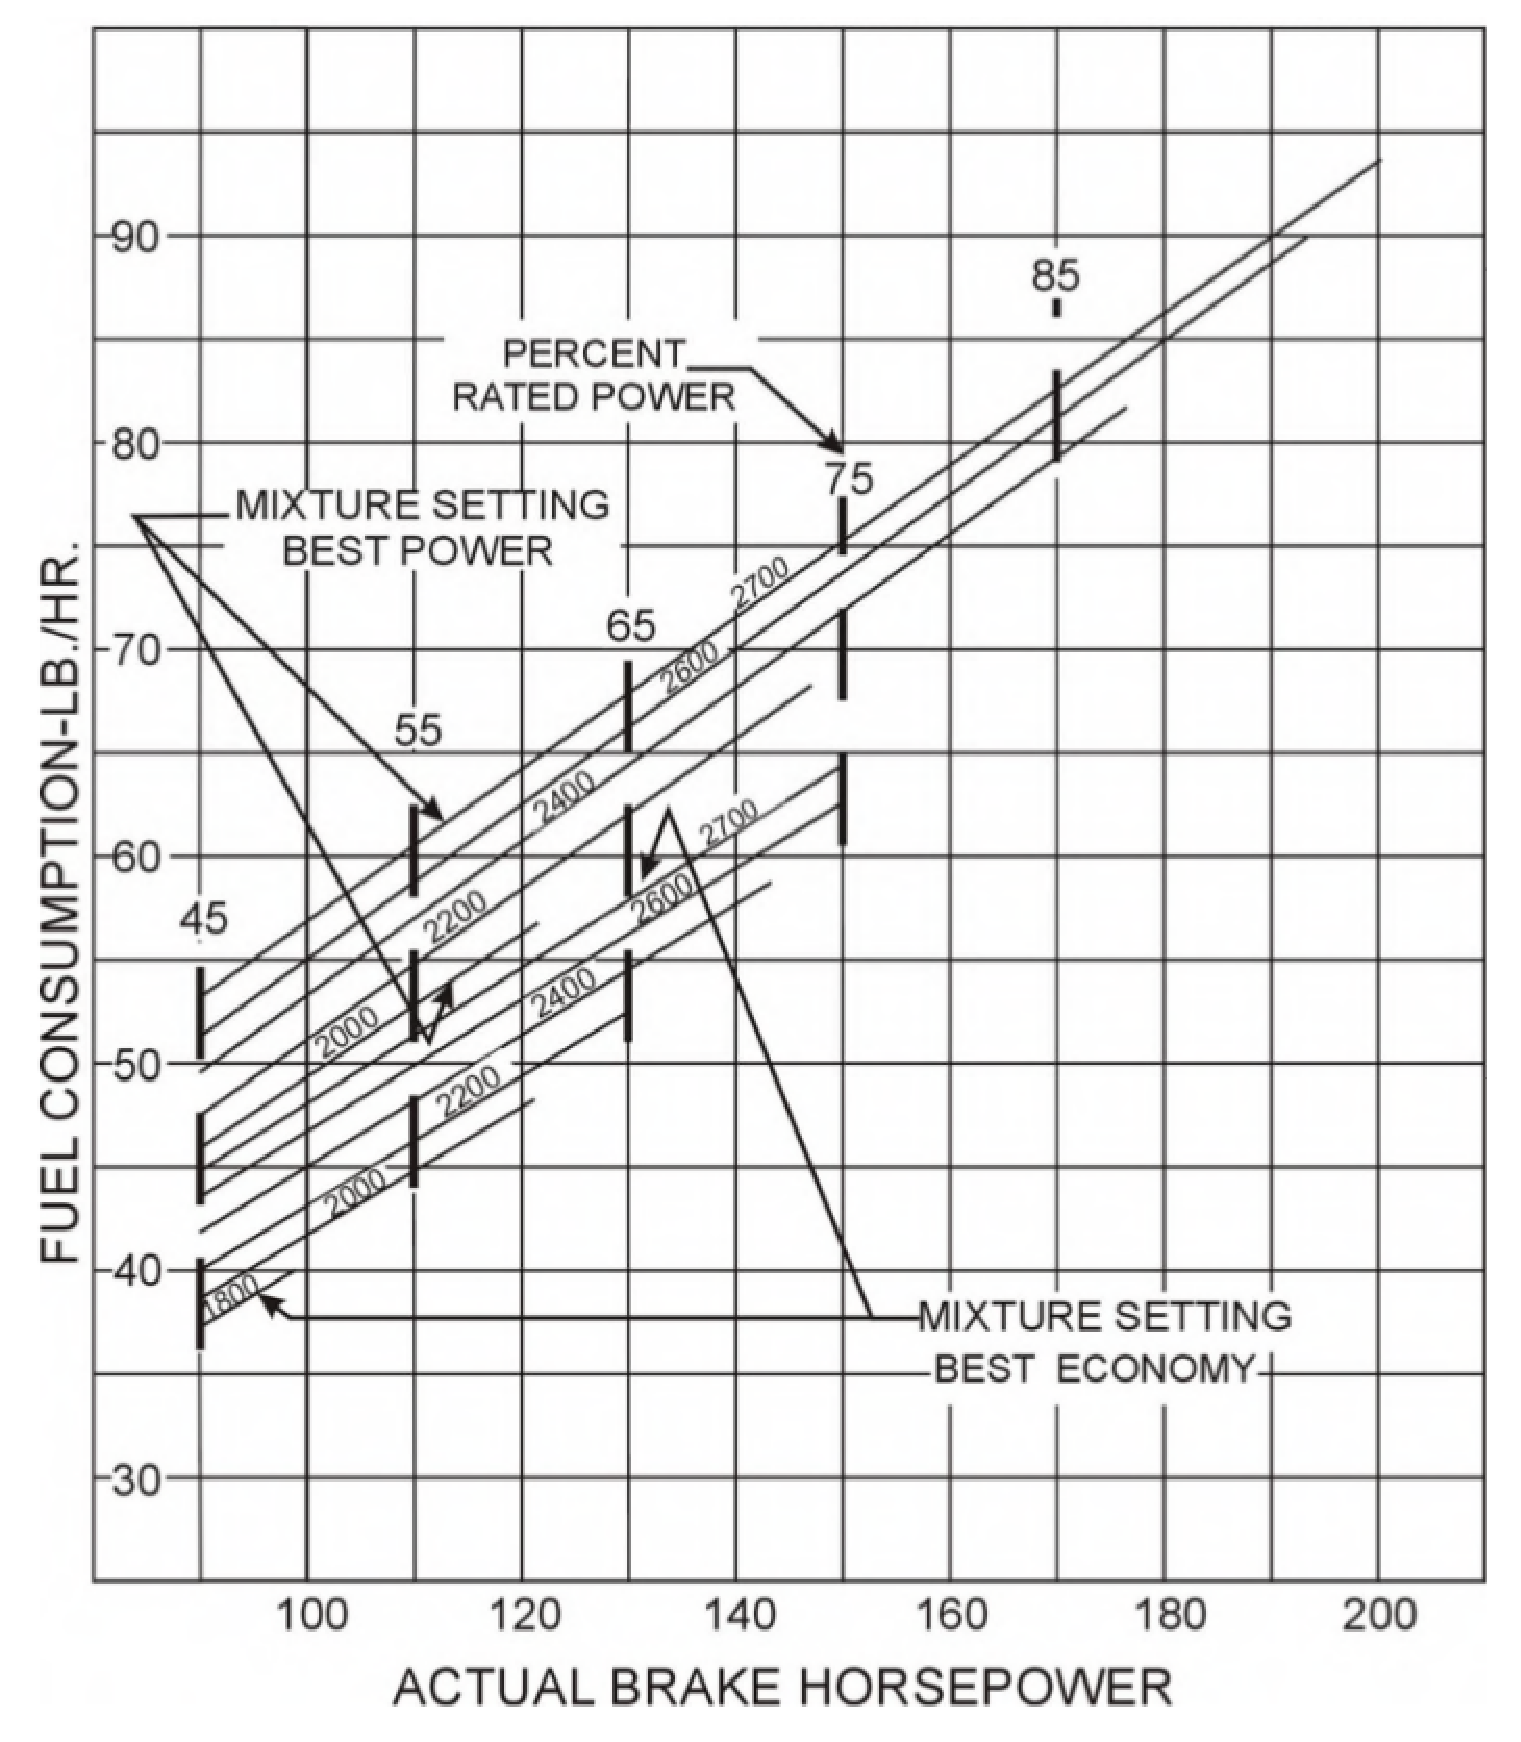
\includegraphics[height=0.\textheight]{IO360-A1B6.eps}
\caption{Fuel consumption for Best Power and Best Economy setting}
\label{fig:fuelflow}
\end{figure}


\section{Cruise performance}
Cruise performance values given below is based on engine power settings alone.  Actual power 
settings depends on environment and altitude of operation. For detailed power settings, please
see Figure \ref{fig:engineperf}.
\begin{table}[h]
\caption{Operating conditions}
\label{tab:performance}
  \begin{tabularx}{\linewidth}{
    |>{\hsize=0.4\hsize}X| 
     >{\hsize=0.2\hsize}X|
     >{\hsize=0.2\hsize}X| 
     >{\hsize=0.2\hsize}X| 
} 
\hline
& RPM & Fuel Flow Gal/Hr. & Oil Use \newline Qts./Hr. \\
\hline
Normal Rated \newline 200 HP & 2700 & 15.4(58.3$\ell$/h) &.89 \\
\hline
Performance Cruise \newline  (75\% Rated) 150 HP & 2450 (23")&  12.3 (47$\ell$/h)  & .50 \\
\hline
Economy Cruise \newline (65\% Rated) 130 HP &  2350 (21") &  9.5 (36 $\ell$/h)&.44 \\
\hline
\end{tabularx}
\end{table}

\begin{figure}[tbh]
  \centering
  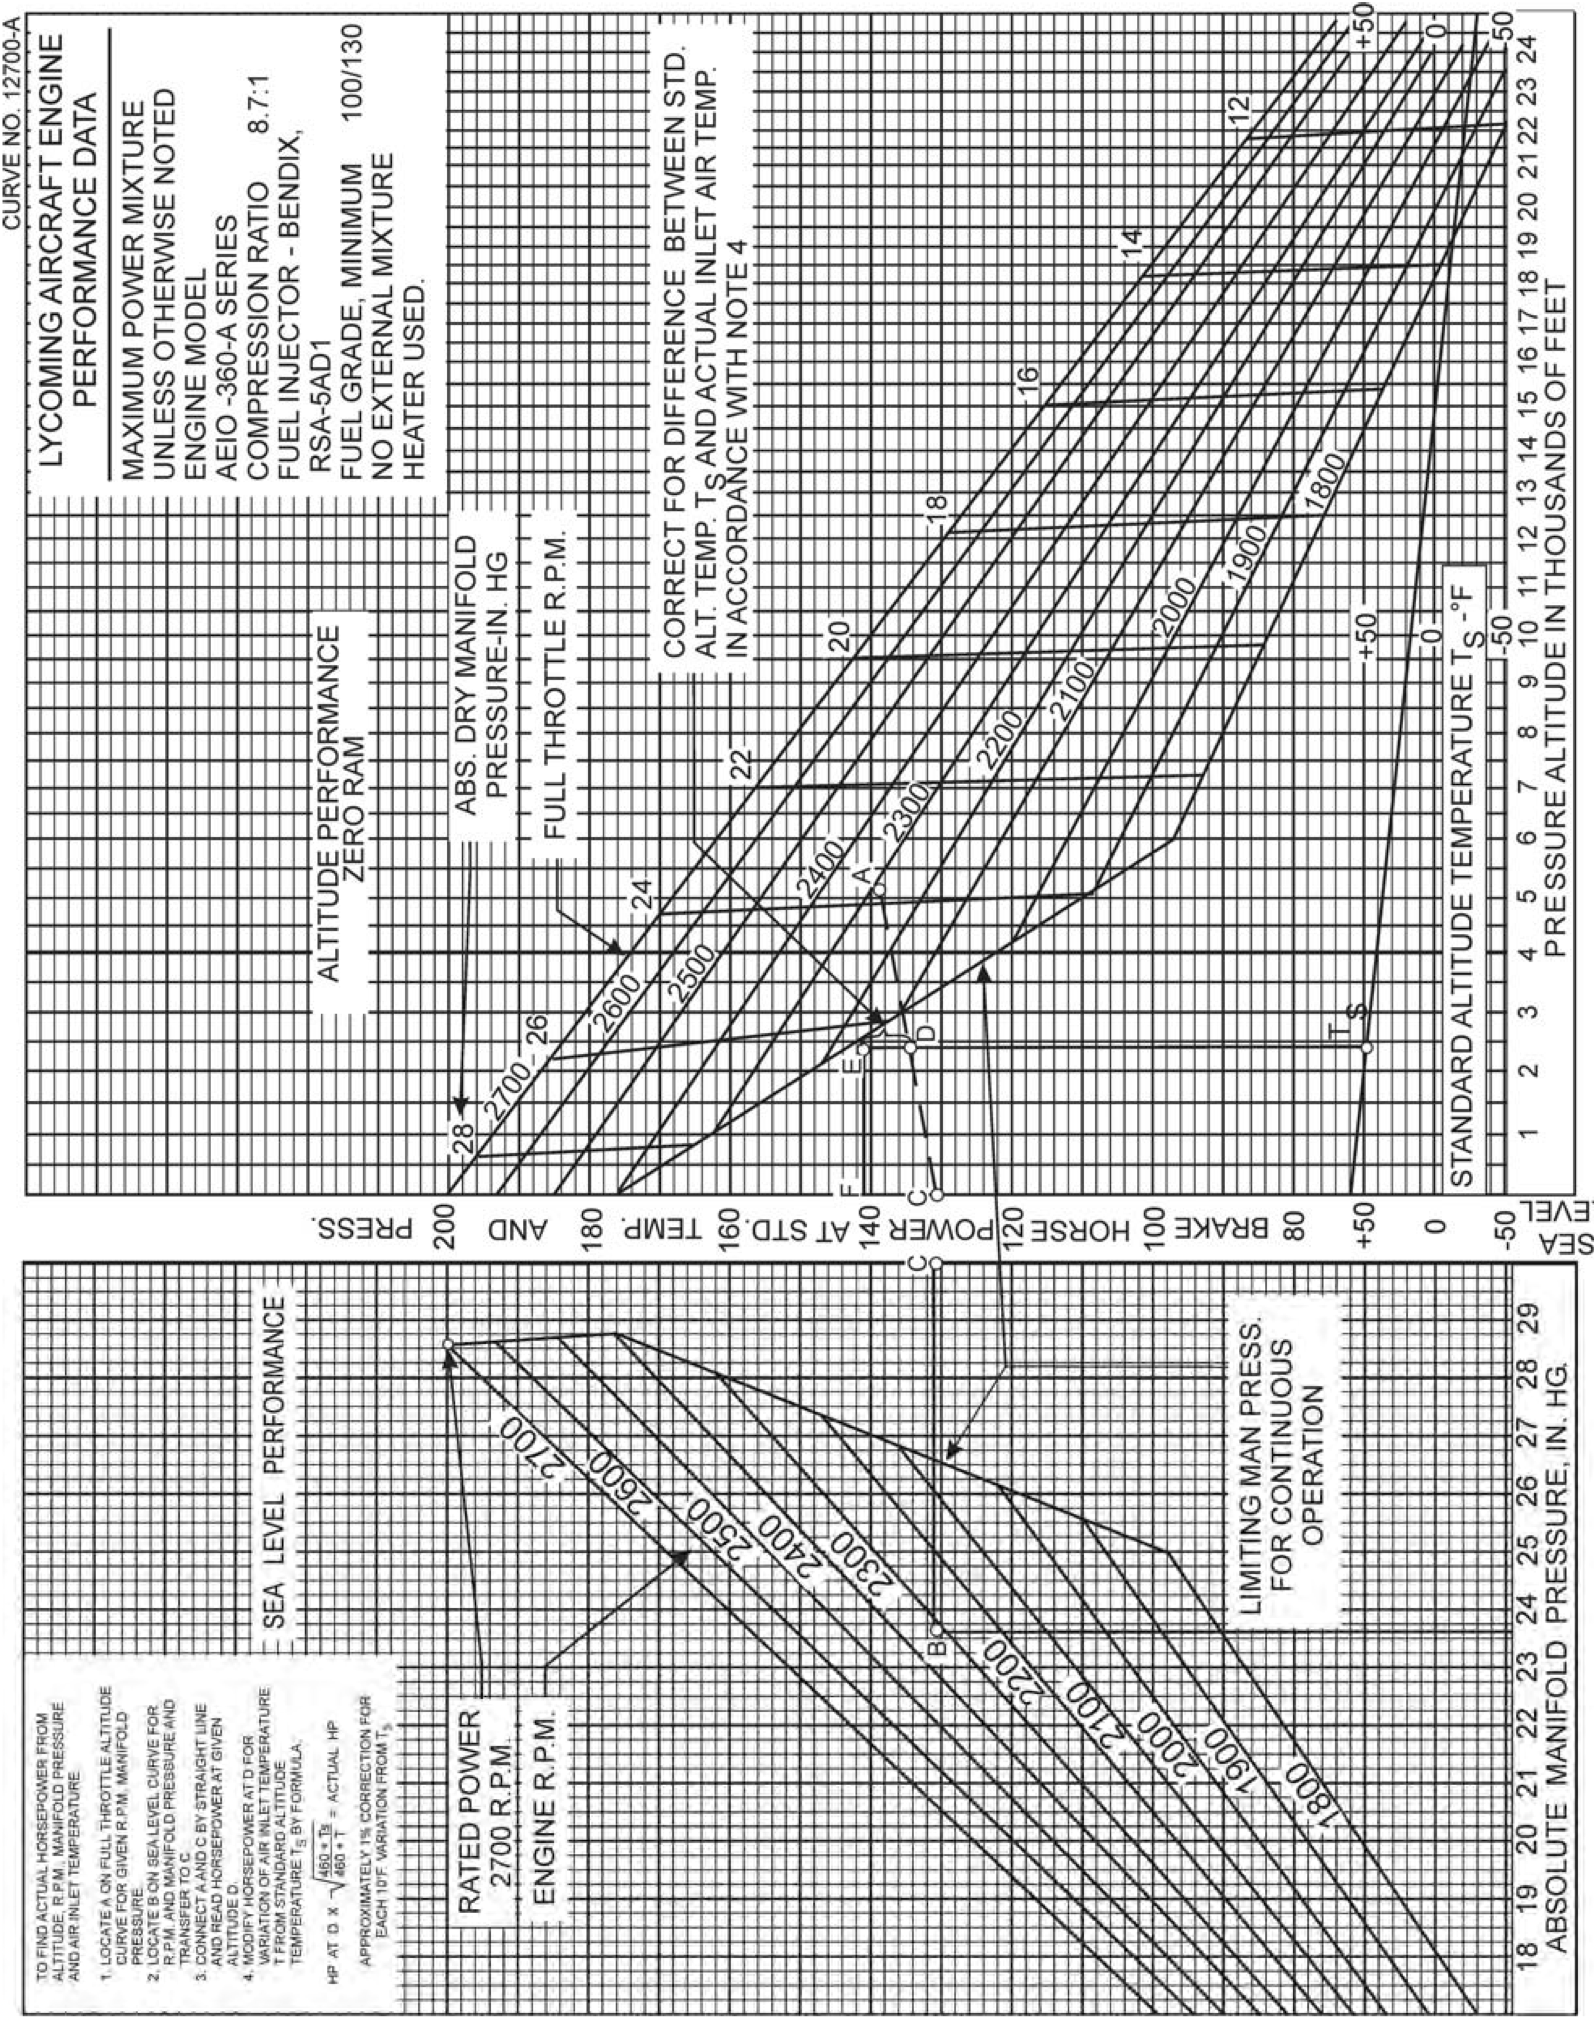
\includegraphics[height=0.9\textheight]{power-settings.png}
  \caption{Engine performance chart}
  \label{fig:engineperf}
\end{figure}

